\subsection{Test framework}
When the HiFi simulation model is initialized, the system takes approximately 1.5 hours until it converges to steady state. Since the optimal controller is not expected to work well when operating far away from the linearisation point, we allow the existing PID control structure to handle the initial transient behavior. It was decided to do this, since making the Simulink project start in steady state would be a manual tedious task.\\


\begin{figure}[h!]
	\centering
	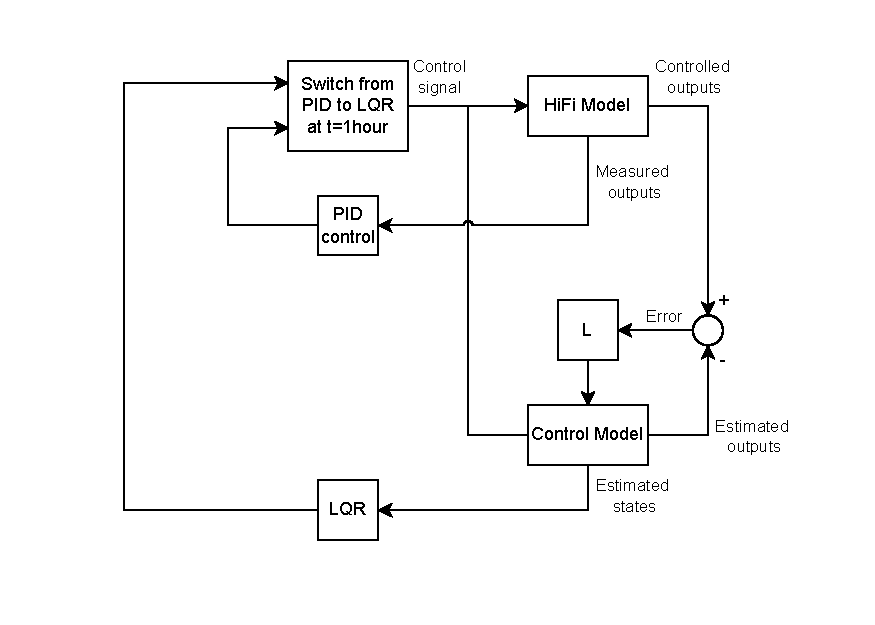
\includegraphics[width=0.8\textwidth]{Graphics/HiFi_simulation_test_diagram.pdf}
	\caption{Top: Cargo hold air temperature. $T_0$ = -4.25$^{\circ}$C. Bottom: Evaporator vapor refrigerant temperature. $T_0$ = -5.55$^{\circ}$C}
	\label{fig:test_setup}
\end{figure}

The test setup is sketched in \cref{fig:test_setup}. A switch is inserted in the simulation which changes the inputs to the Hi-Fi simulation from the PID control structure to the LQR controller at some specified time. It takes two inputs: the vector of the PID chosen control inputs and the vector of the LQR controller input. The PID inputs are fed to the system until the time reaches 1 hour. At this point, the switch selects the LQR control inputs to be fed to the system. Until the switching time, the control model states are forced to stay at 0.\\

Two simulations will run in parallel: The above described, and one where the PID controller continues to regulate the system for the entire simulation. This allows for comparison between the two control strategies. \\


\subsection{Tuned LQR controller: Constant disturbance}
The LQR controller is set to start regulating the system at time $t=1.1$ hours, at which point it will attempt drive the states to 0. The disturbance (ambient temperature) is held constant at 20$^{\circ}$C. This is the operating point for the disturbance, and will thus not affect the system. The controlled outputs are seen in \cref{fig:LQR_wellTuned_noDist}.\\


\begin{figure}[H]
	\centering
	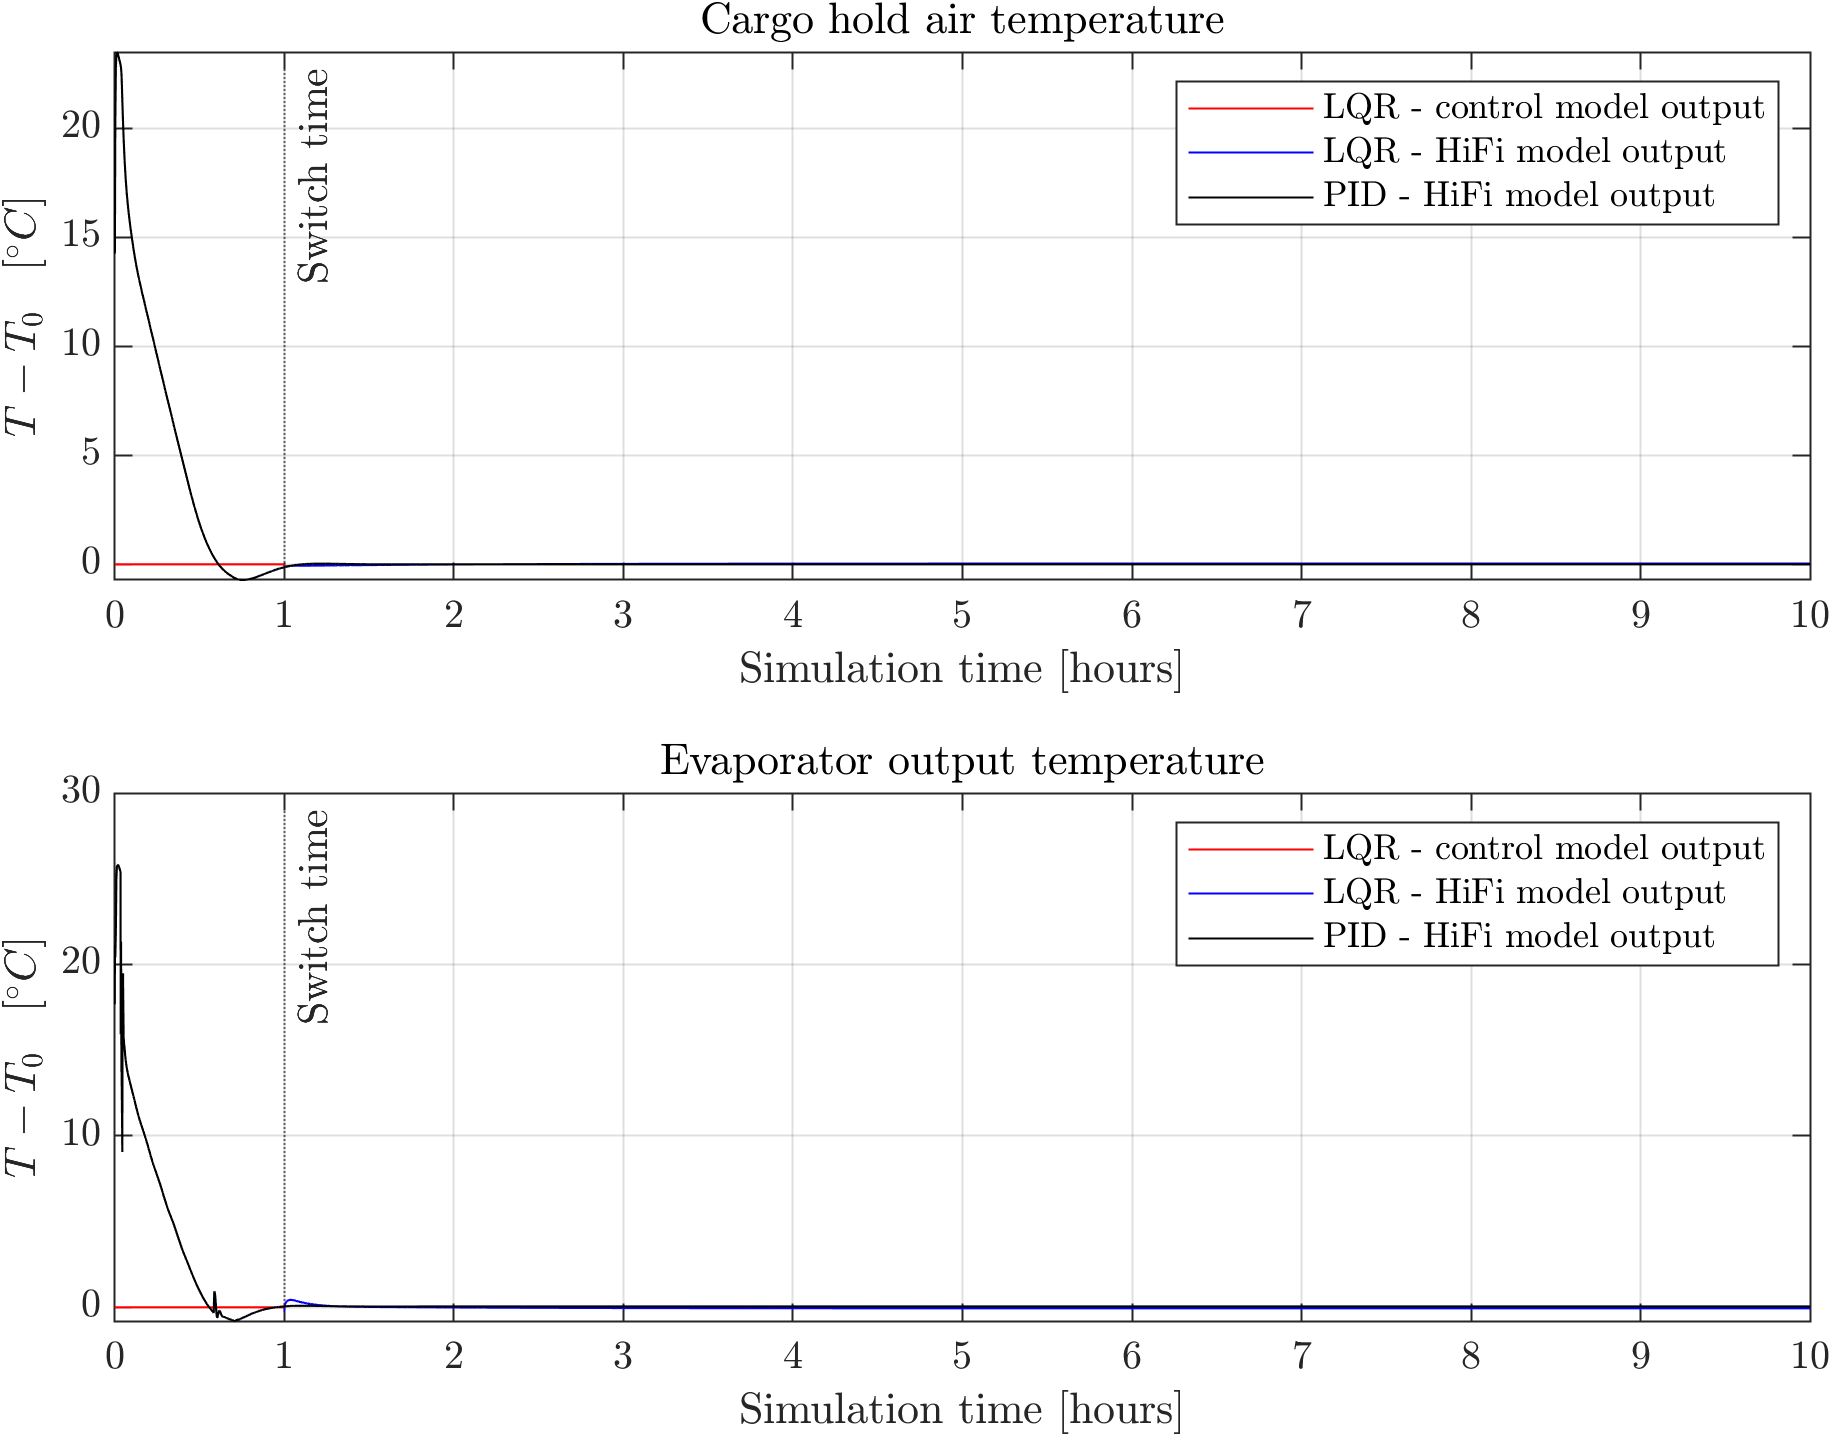
\includegraphics[width=0.8\textwidth]{Graphics/fig_LQRvsKresten_noDist.png}
	\caption{Top: Cargo hold air temperature. $T_0$ = -4.25$^{\circ}$C. Bottom: Evaporator vapor refridgerant temperature. $T_0$ = -5.55$^{\circ}$C\\\hspace{\textwidth} During the initial transient phase the estimated }
	\label{fig:LQR_wellTuned_noDist}
\end{figure}

\cref{fig:LQR_wellTuned_noDist_zoom} shows a zoomed in version of \cref{fig:LQR_wellTuned_noDist}, where the steady state error of the two outputs is seen.\\


\begin{figure}[H]
	\centering
	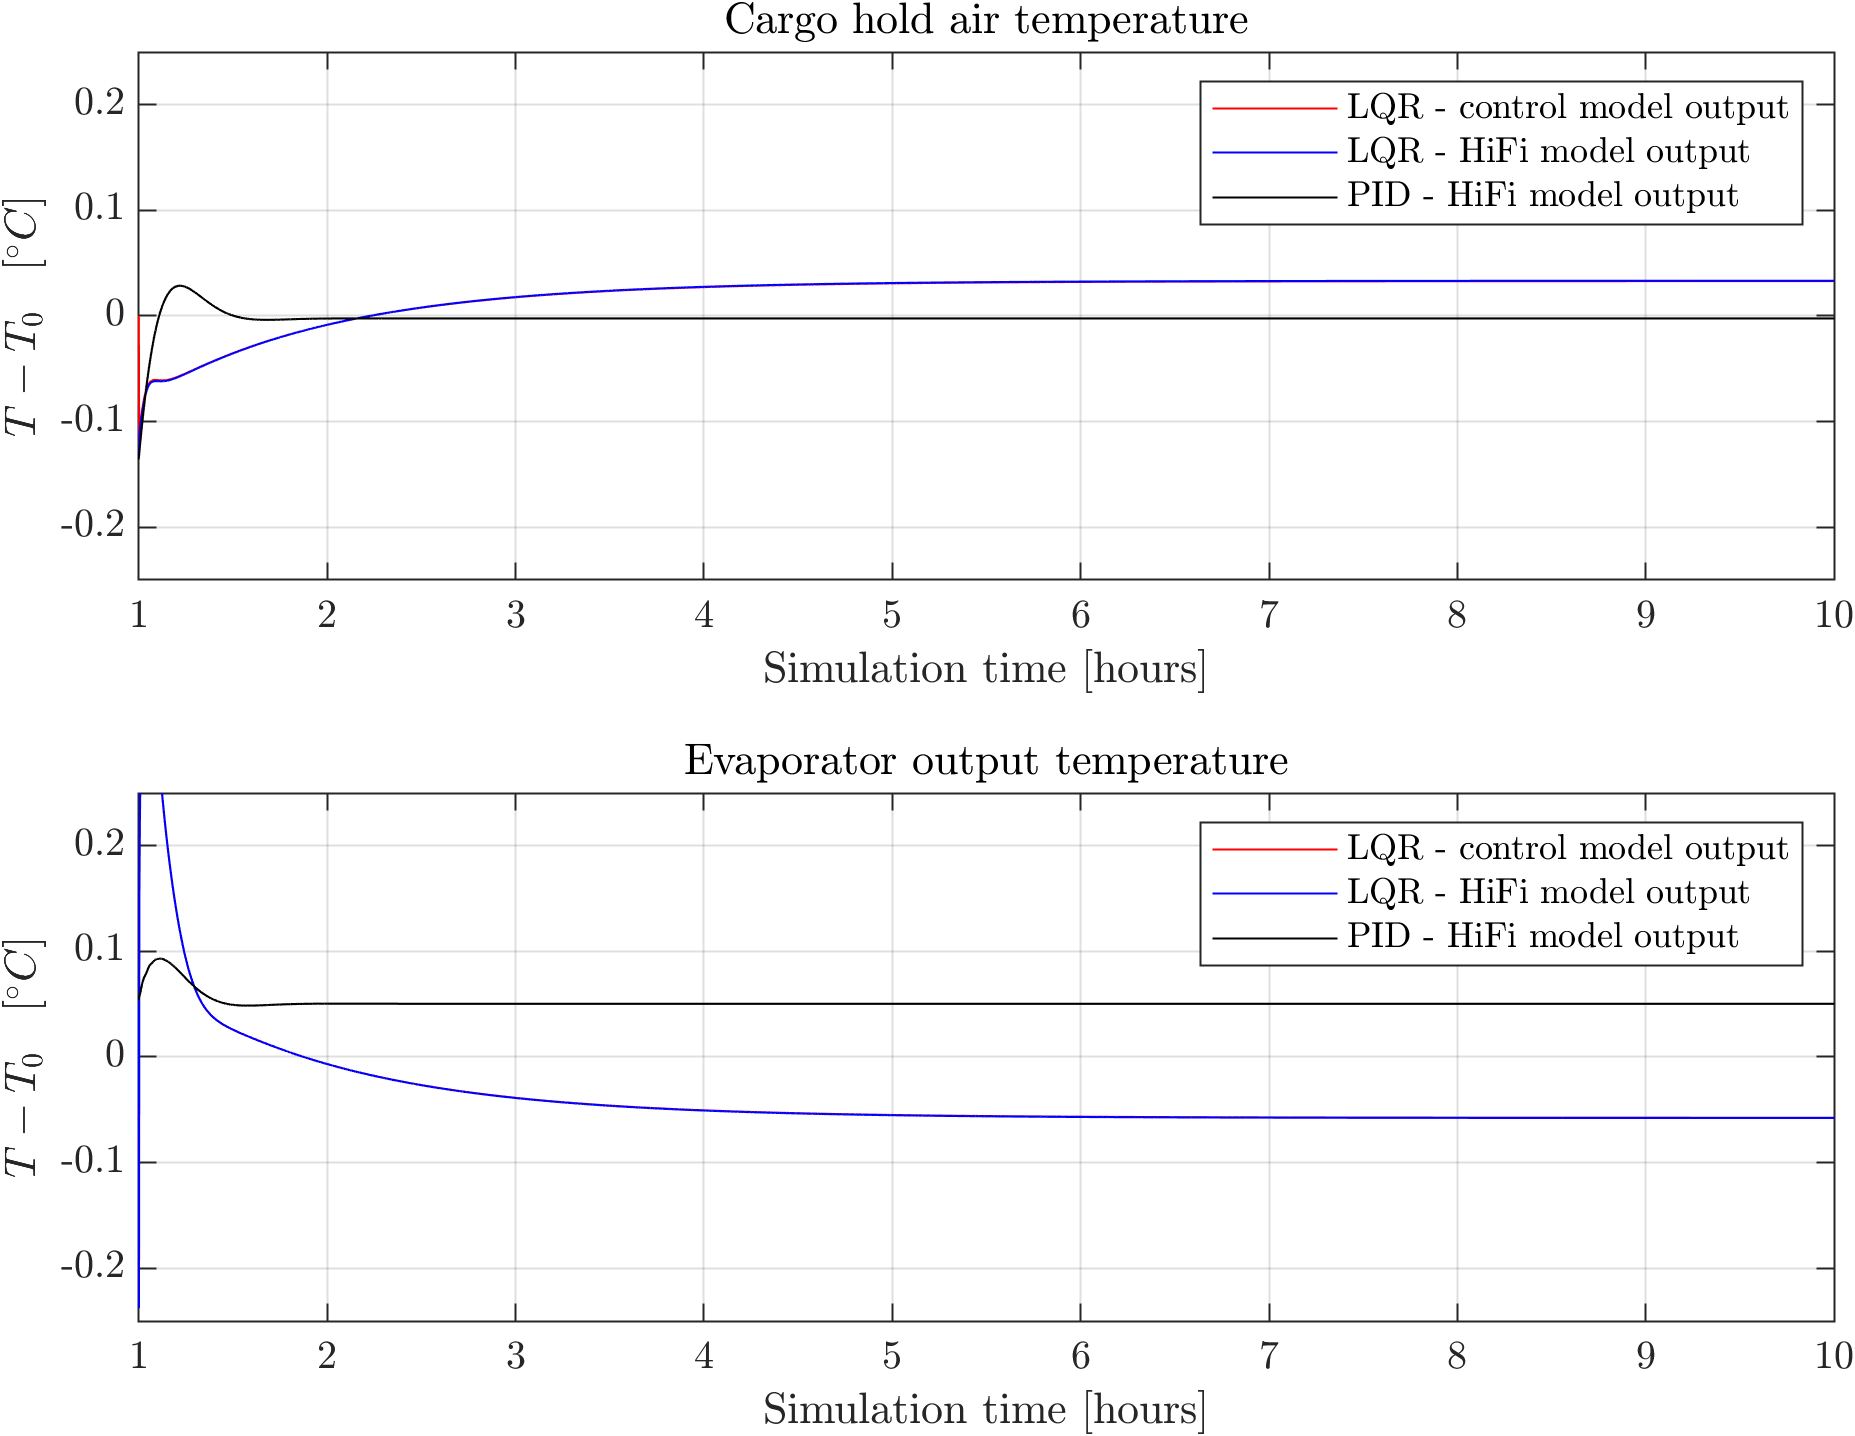
\includegraphics[width=0.8\textwidth]{Graphics/fig_LQRvsKresten_noDist_zoom.png}
	\caption{Top: Cargo hold air temperature. $T_0$ = -4.25$^{\circ}$C. Bottom: Evaporator vapor refridgerant temperature. $T_0$ = -5.55$^{\circ}$C}
	\label{fig:LQR_wellTuned_noDist_zoom}
\end{figure}

The error is so numerically small that most real temperature sensors would be unable to detect it. The LQR controller is thus shown to be able to drive the system to practically zero, when no disturbance is present. The settling time is however noticeably longer than that of the PID controlled system.  \\

The control inputs during this test is seen in \cref{fig:inputs_noDist}.

\begin{figure}[H]
	\centering
	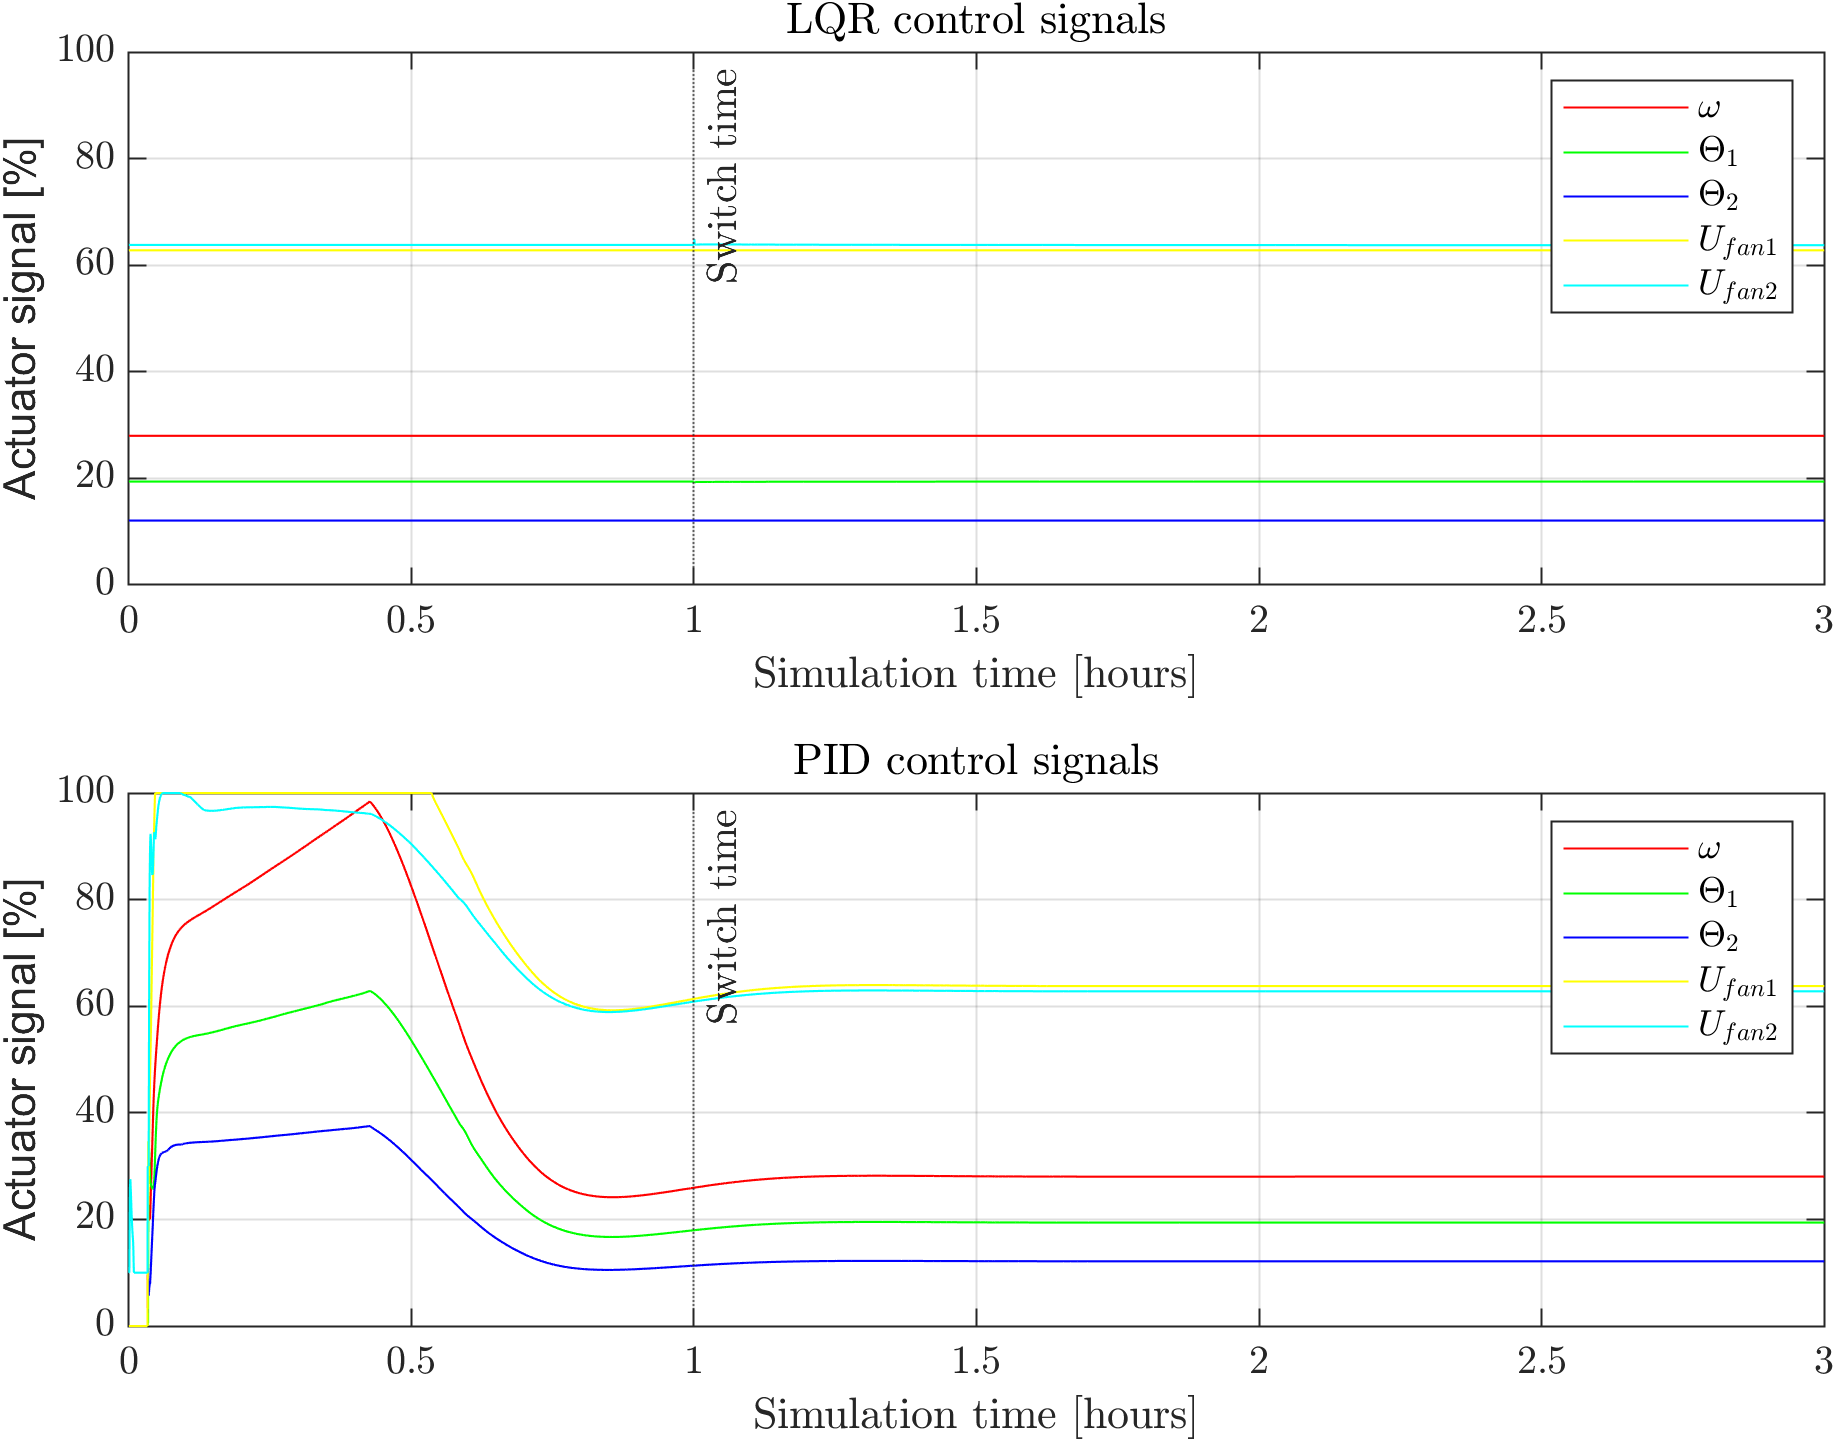
\includegraphics[width=0.8\textwidth]{Graphics/fig_inputs_noDist.png}
	\caption{text}
	\label{fig:inputs_noDist}
\end{figure}

\begin{figure}[H]
	\centering
	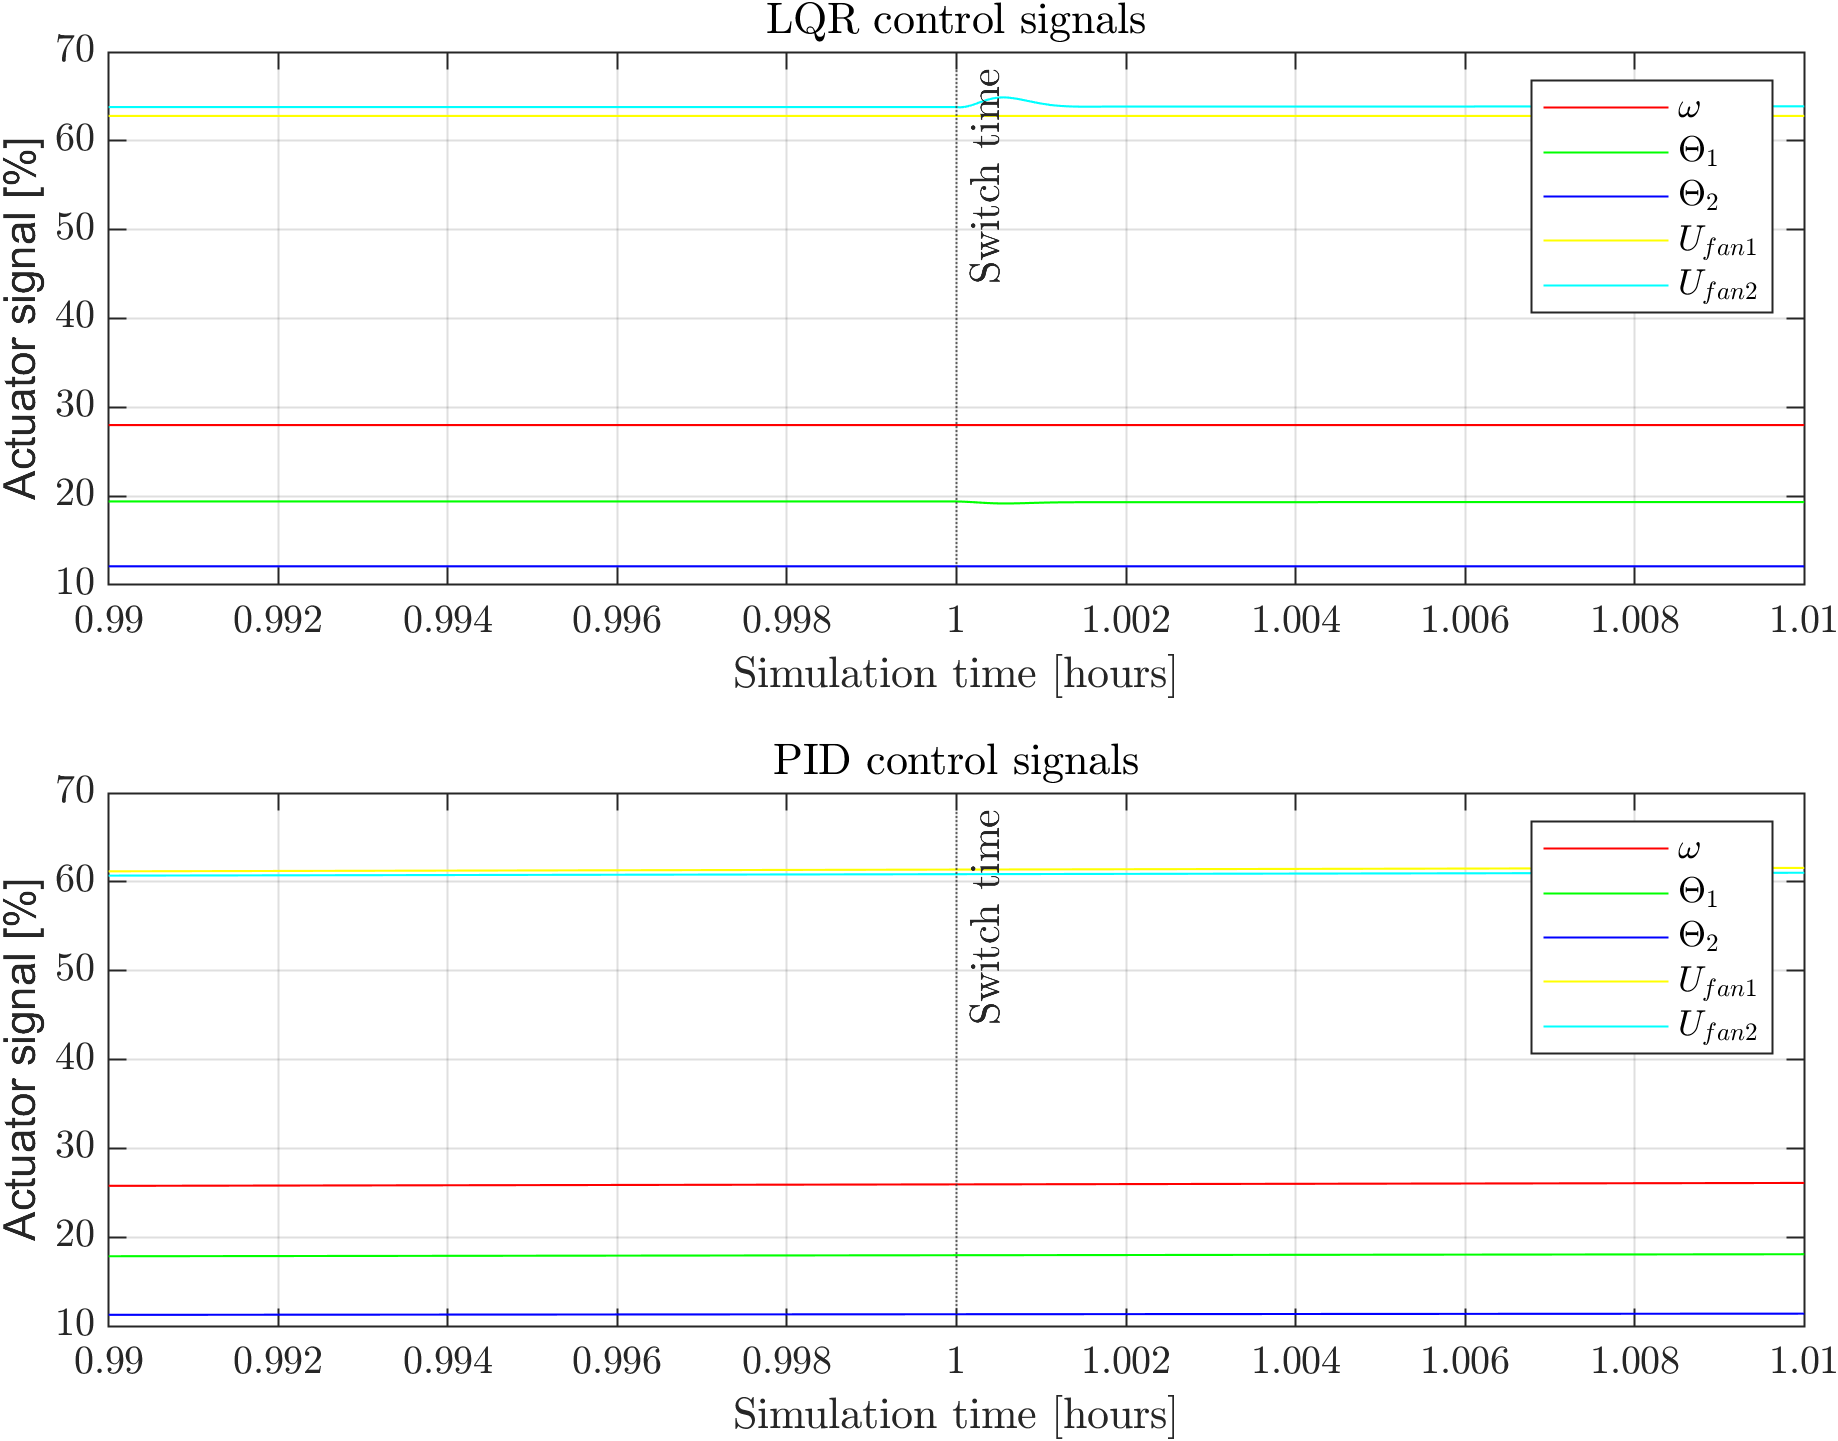
\includegraphics[width=0.8\textwidth]{Graphics/fig_inputs_noDist_zoom.png}
	\caption{text}
	\label{fig:inputs_noDist_zoom}
\end{figure}

\newpage
\subsection{Tuned LQR controller: Sine disturbance}
We will now investigate the dymanic controller performance when a sine disturbance is applied to the system. As before, PID controller will handle the initial hour of settling. The LQR then starts regulating the system, and at time $t=3$ hours, the a disturbance is injected to the ambient temperature. The disturbance is a sine wave with an amplitude of 5$^{\circ}$C and a period of 10 minuttes. The controlled outputs are seen in \cref{fig:LQR_wellTuned_sineDist}.\\


\begin{figure}[H]
	\centering
	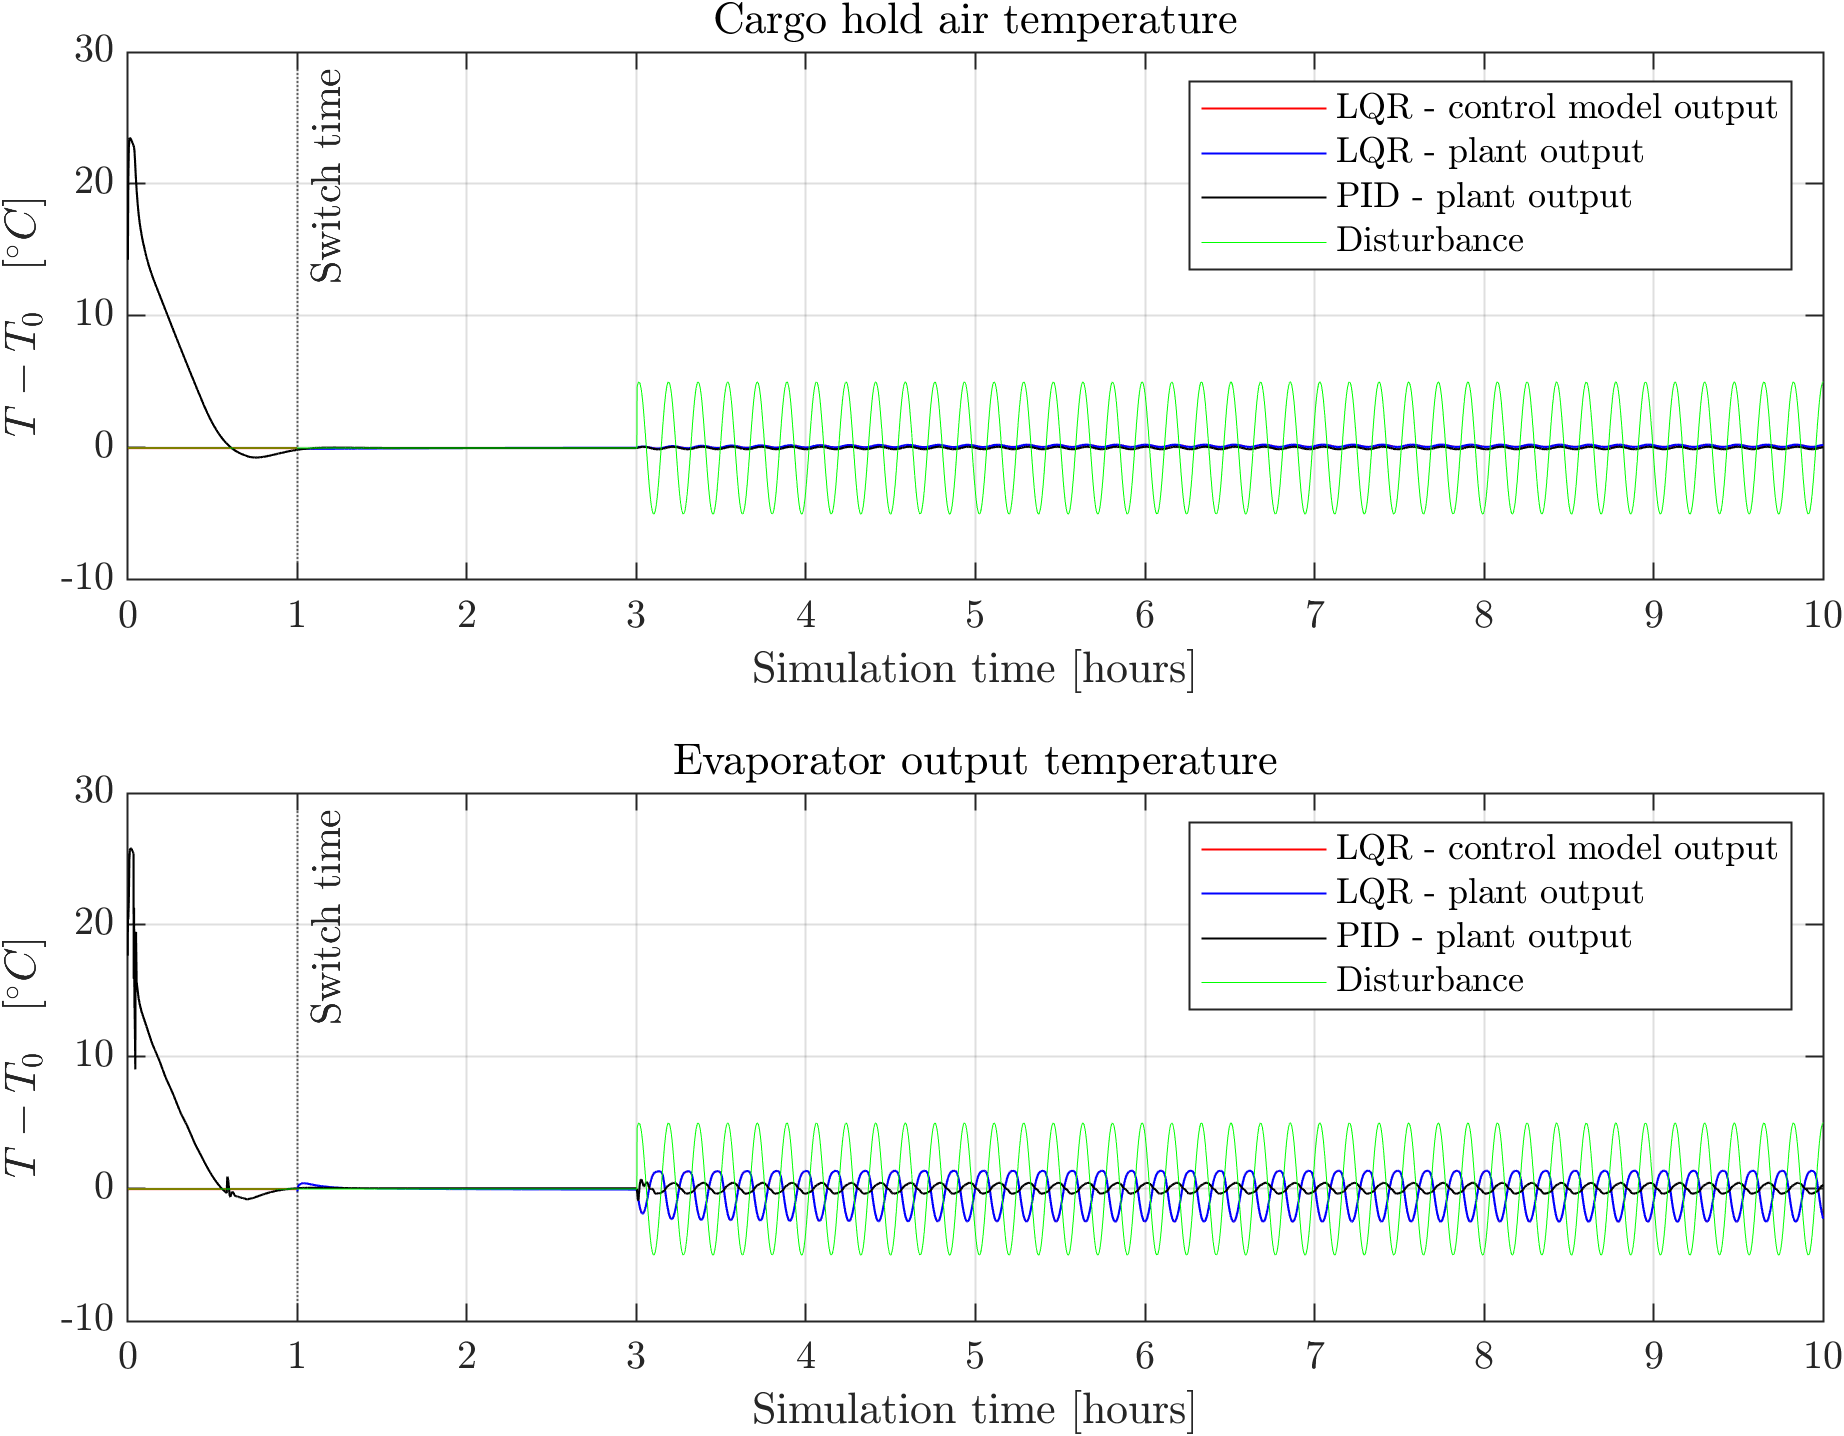
\includegraphics[width=0.8\textwidth]{Graphics/fig_LQRvsKresten_sineDist.png}
	\caption{Top: Cargo hold air temperature. $T_0$ = -4.25$^{\circ}$C. Bottom: Evaporator vapor refridgerant temperature. $T_0$ = -5.55$^{\circ}$C}
	\label{fig:LQR_wellTuned_sineDist}
\end{figure}

\cref{fig:LQR_wellTuned_sineDist_zoom} shows a zoomed in version of \cref{fig:LQR_wellTuned_sineDist}, where the steady state behavior of the two outputs is seen.\\


\begin{figure}[H]
	\centering
	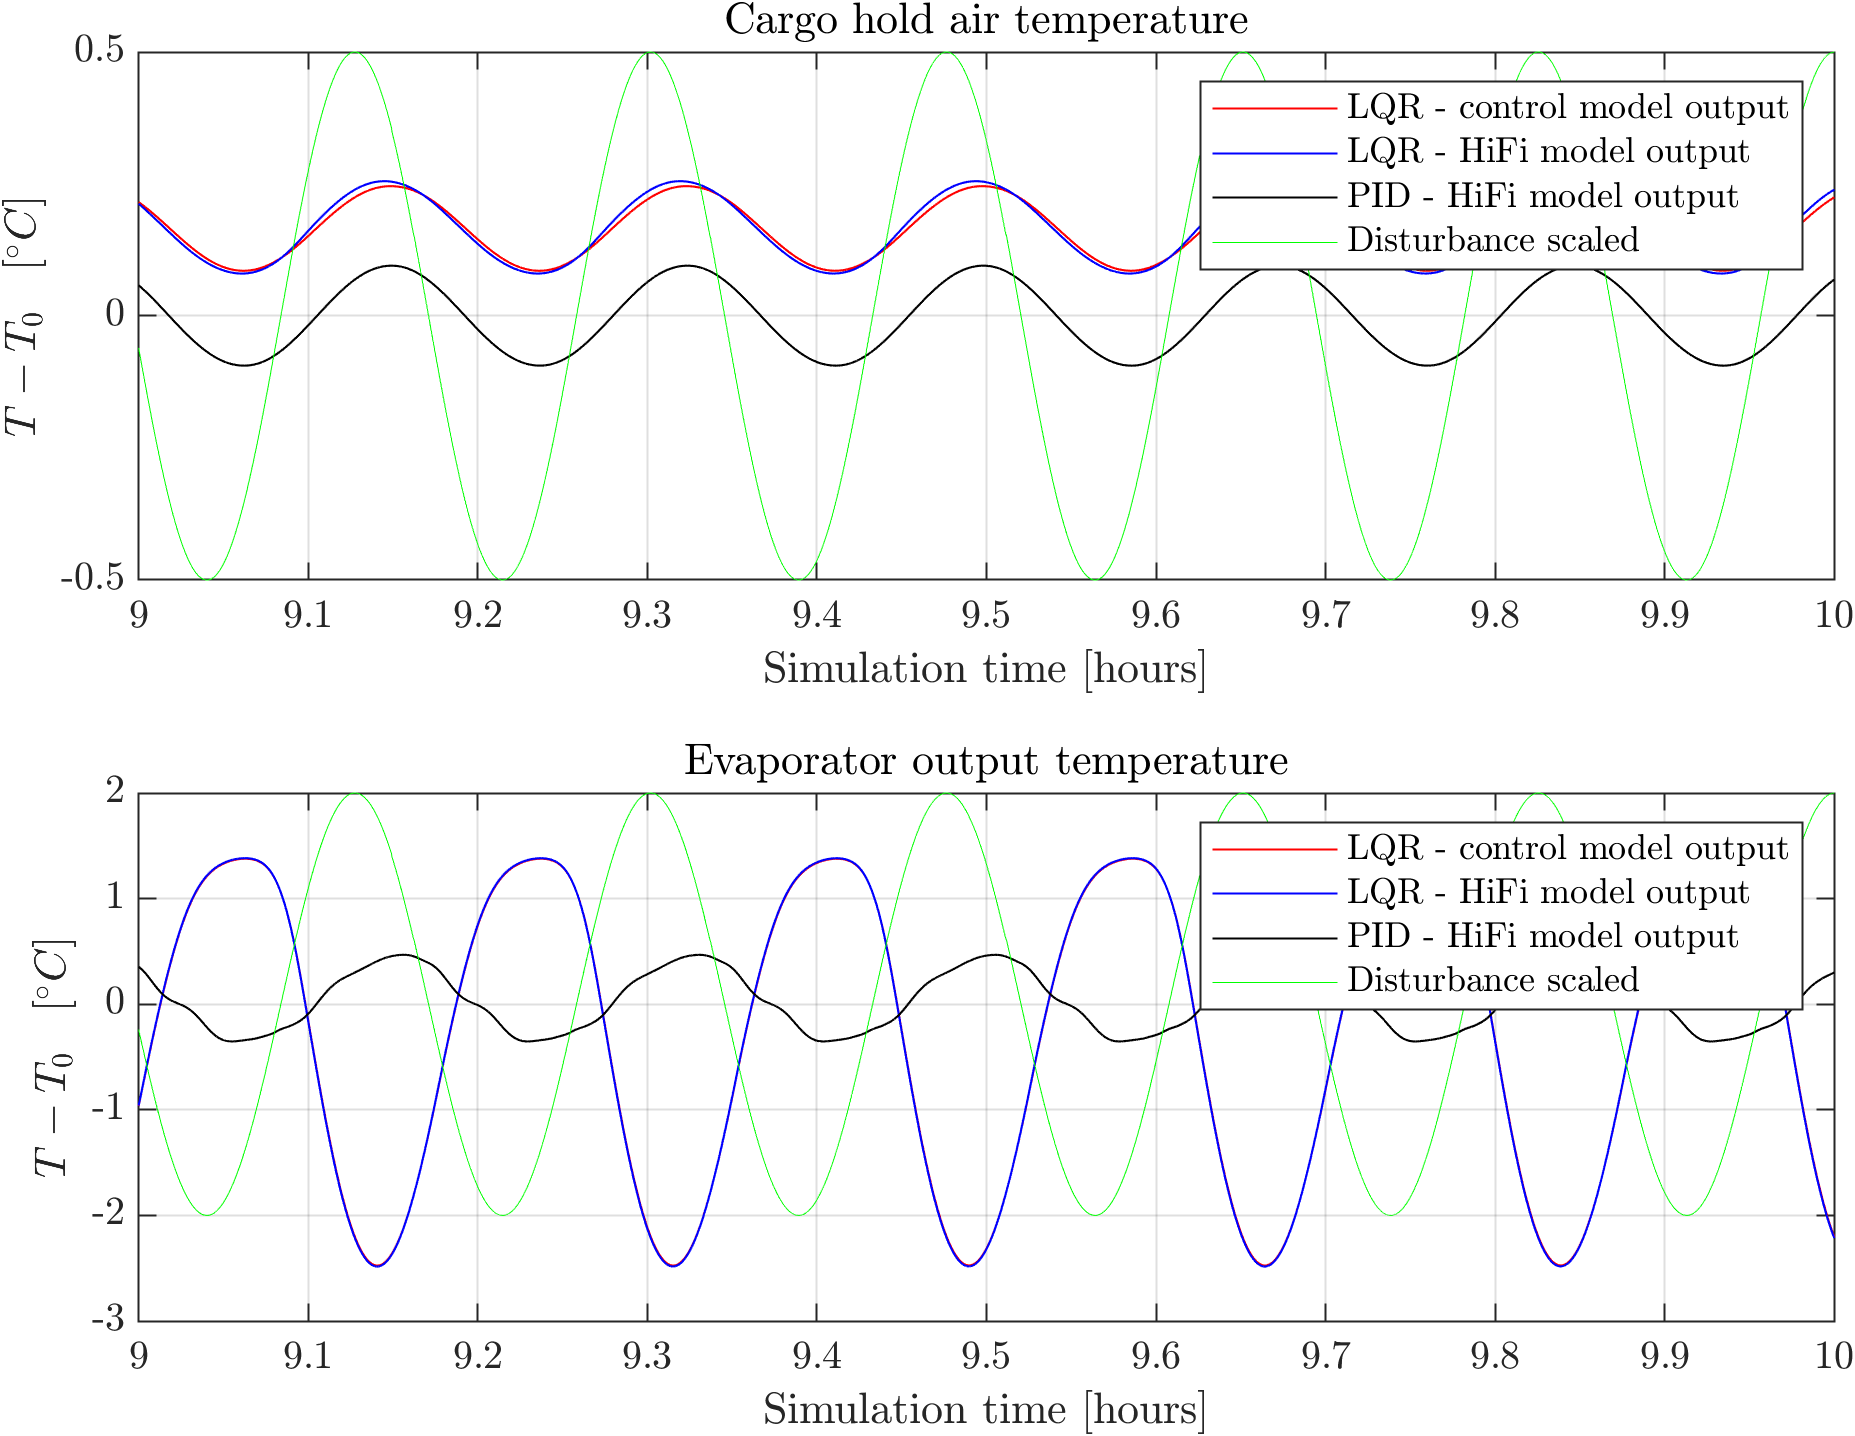
\includegraphics[width=0.8\textwidth]{Graphics/fig_LQRvsKresten_sineDist_zoom.png}
	\caption{Top: Cargo hold air temperature. $T_0$ = -4.25$^{\circ}$C. Bottom: Evaporator vapor refrigerant temperature. $T_0$ = -5.55$^{\circ}$C}
	\label{fig:LQR_wellTuned_sineDist_zoom}
\end{figure}

A few interesting things are revealed in these plots. Firstly, the amplitude of the oscillations of $T_v$ are considerably lower with the PID control structure, than with the LQR controller. This implies that the optimal control strategy is less keen to correct for errors on that particular state. Intuitively this would be improved by penalizing the relevant entry in the $Q$ weighing matrix. This has been attempted, and it was found that increasing the weight led to larger oscillations in the state. \\

It is likely that the main cause of this phenomenon, is the control model itself. Due to the simplifications made, and the Kalman decomposition, information about the unused inputs' ($\omega$, $U_{fan_1}$ and $\theta_2$) effect on the states was lost. It is expected that a controller (such as the PID structure), that is able to regulate these inputs would perform better, i.e. minimize the oscillations.\\

The oscillations on the cargo hold air temperature are not visibly different for the two control strategies. The amplitude of the oscillation is 0.18$^{\circ}$C. Thus the control strategy is performing well at minimizing an oscillating ambient temperatures effect on the air temperature inside the trailer. \\

The control inputs during this test is seen in \cref{fig:inputs_sineDist}.

\begin{figure}[H]
	\centering
	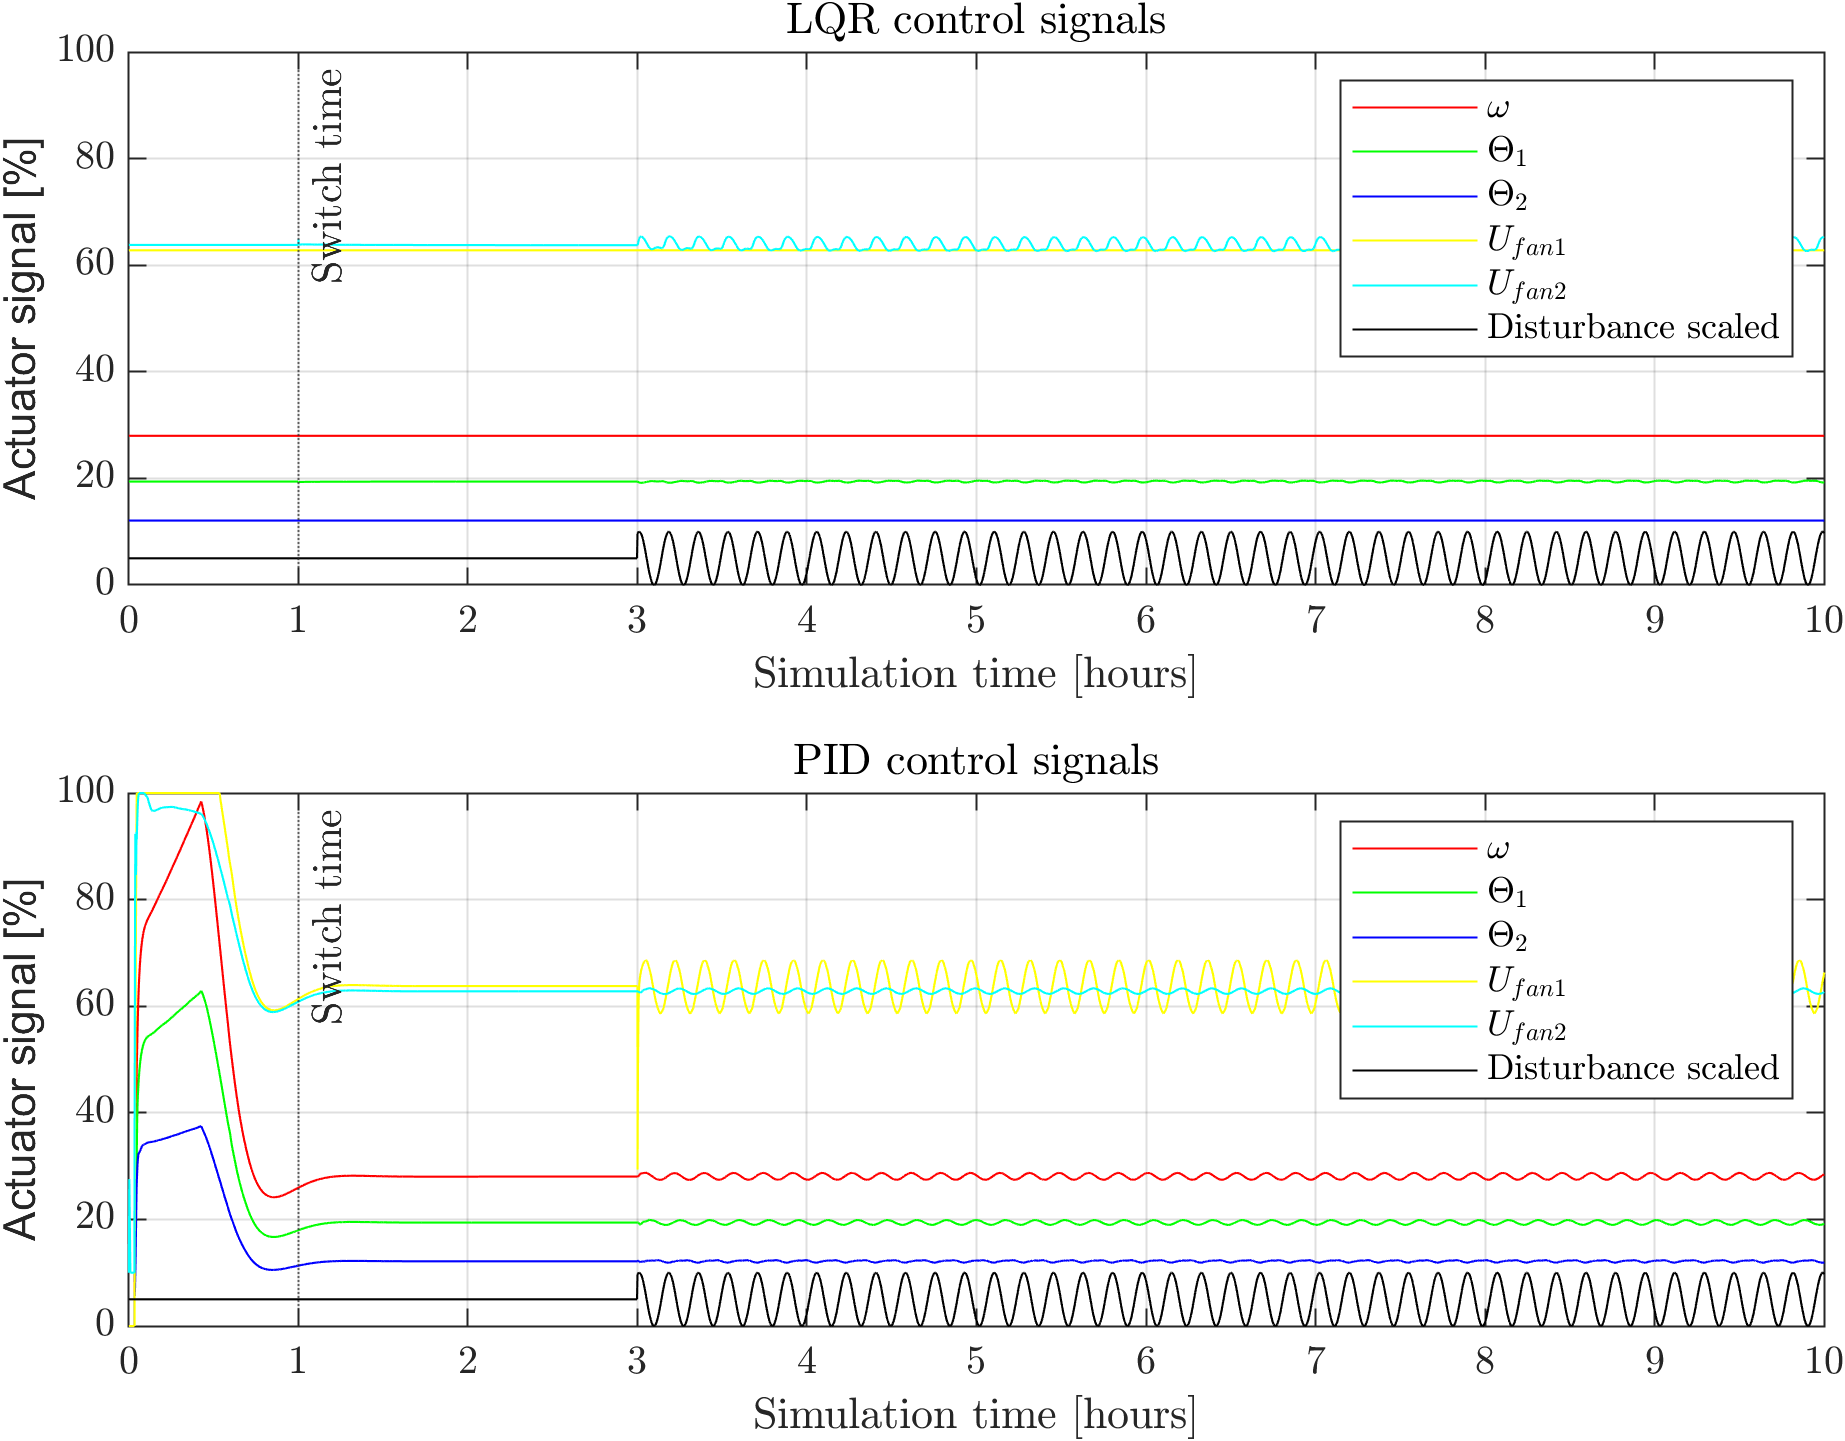
\includegraphics[width=0.8\textwidth]{Graphics/fig_inputs_sineDist.png}
	\caption{text}
	\label{fig:inputs_sineDist}
\end{figure}

\begin{figure}[H]
	\centering
	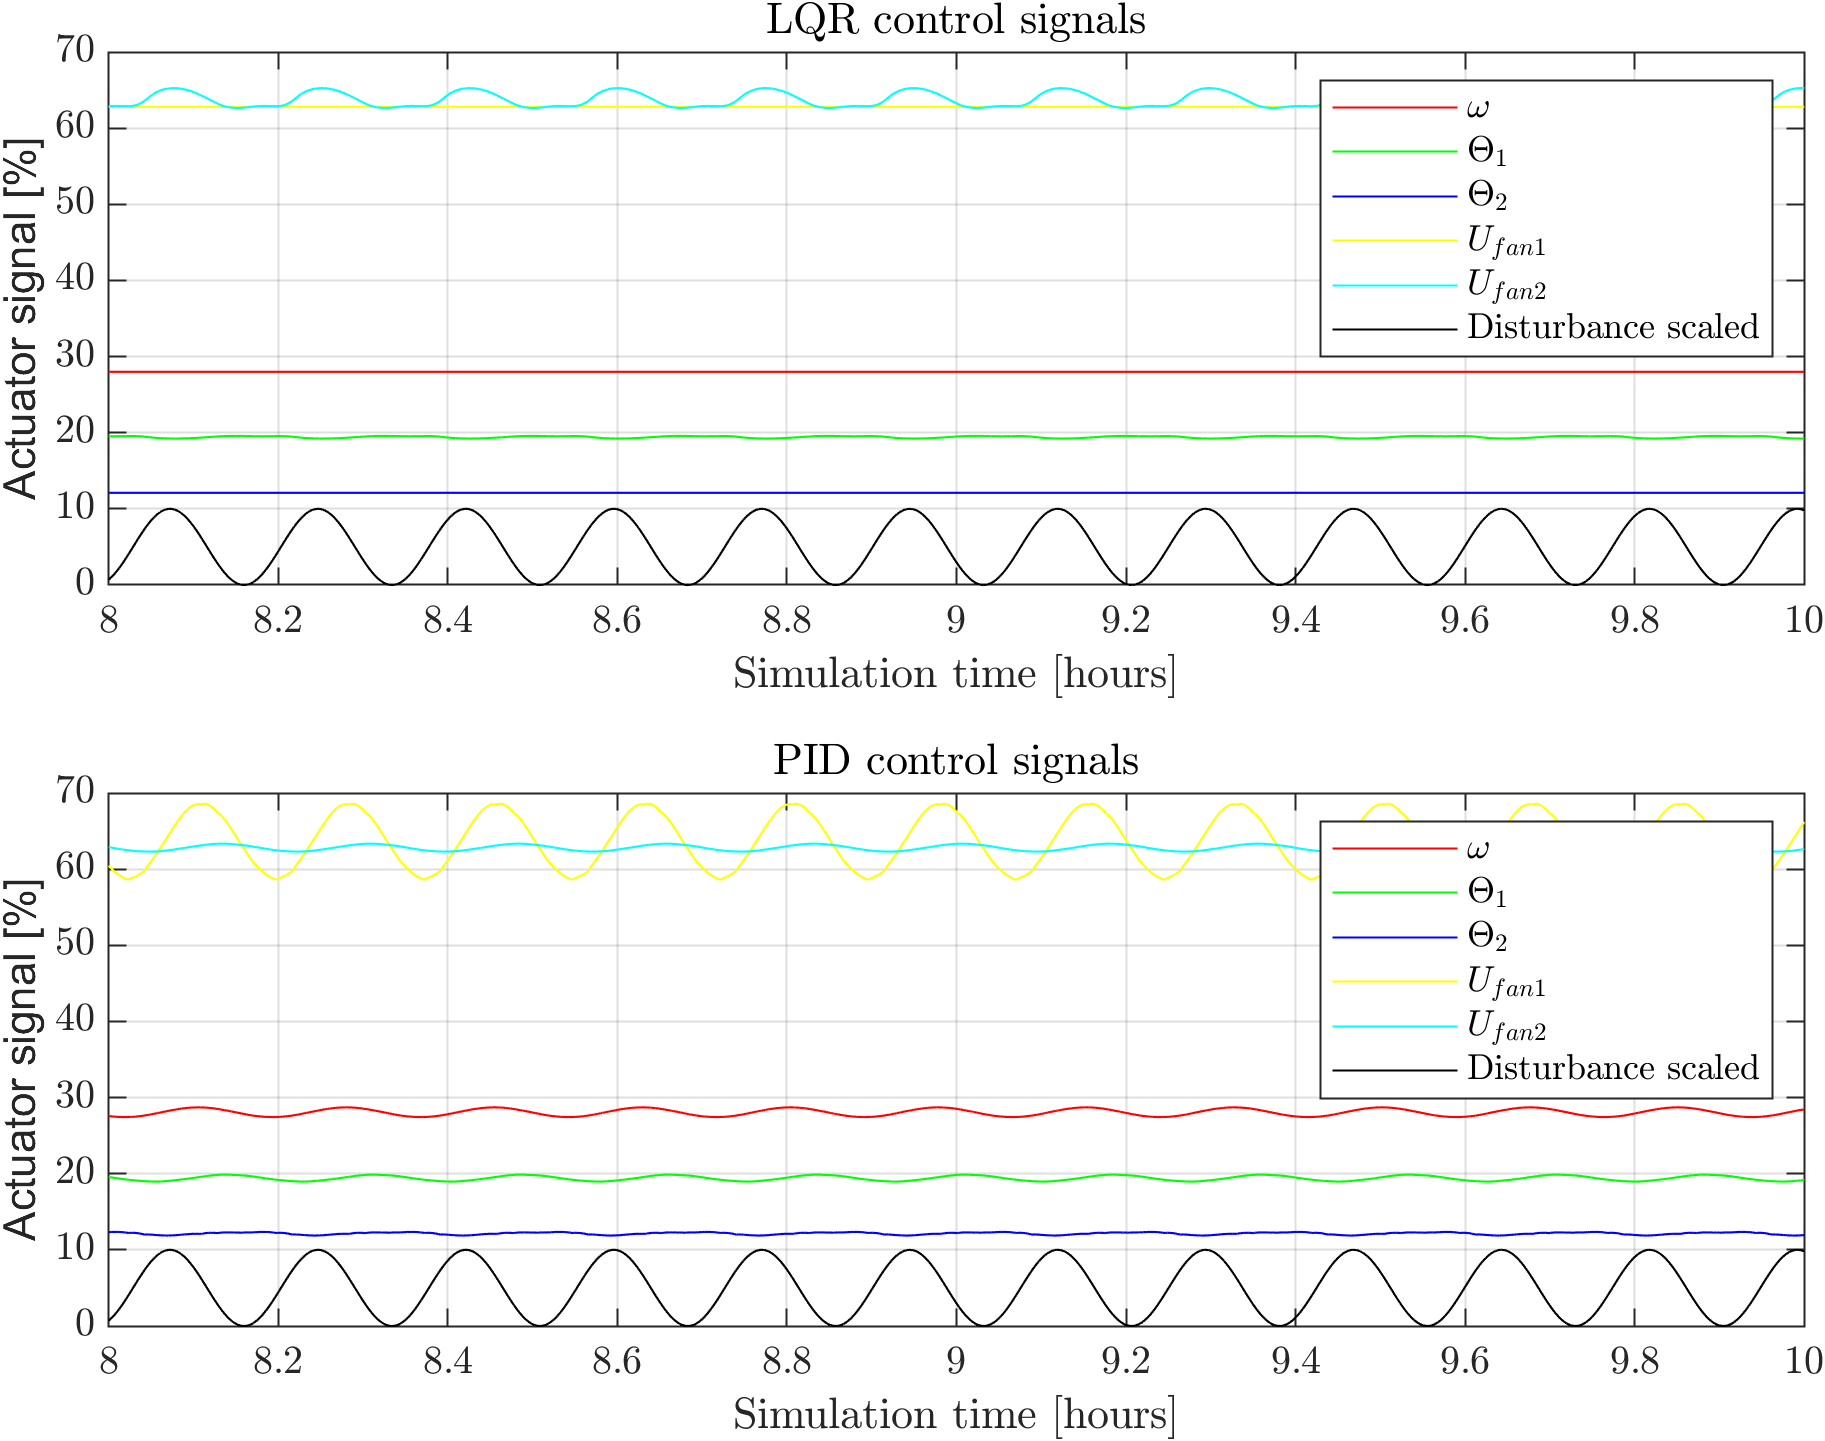
\includegraphics[width=0.8\textwidth]{Graphics/fig_inputs_sineDist_zoom.png}
	\caption{text}
	\label{fig:inputs_sineDist_zoom}
\end{figure}


\newpage
\subsection{Tuned LQR controller: Step disturbance}
To test the models ability to continuously perform outside the operating point, a step disturbance is applied to the ambient temperature.  At time $t=3$ hours, a 5$^{\circ}$C step in the disturbance is introduced. As before the PID structure handles the first hour of simulation, after which the optimal controller takes action. The controlled outputs are seen in \cref{fig:LQR_wellTuned_5stepDist}.\\

\begin{figure}[H]
	\centering
	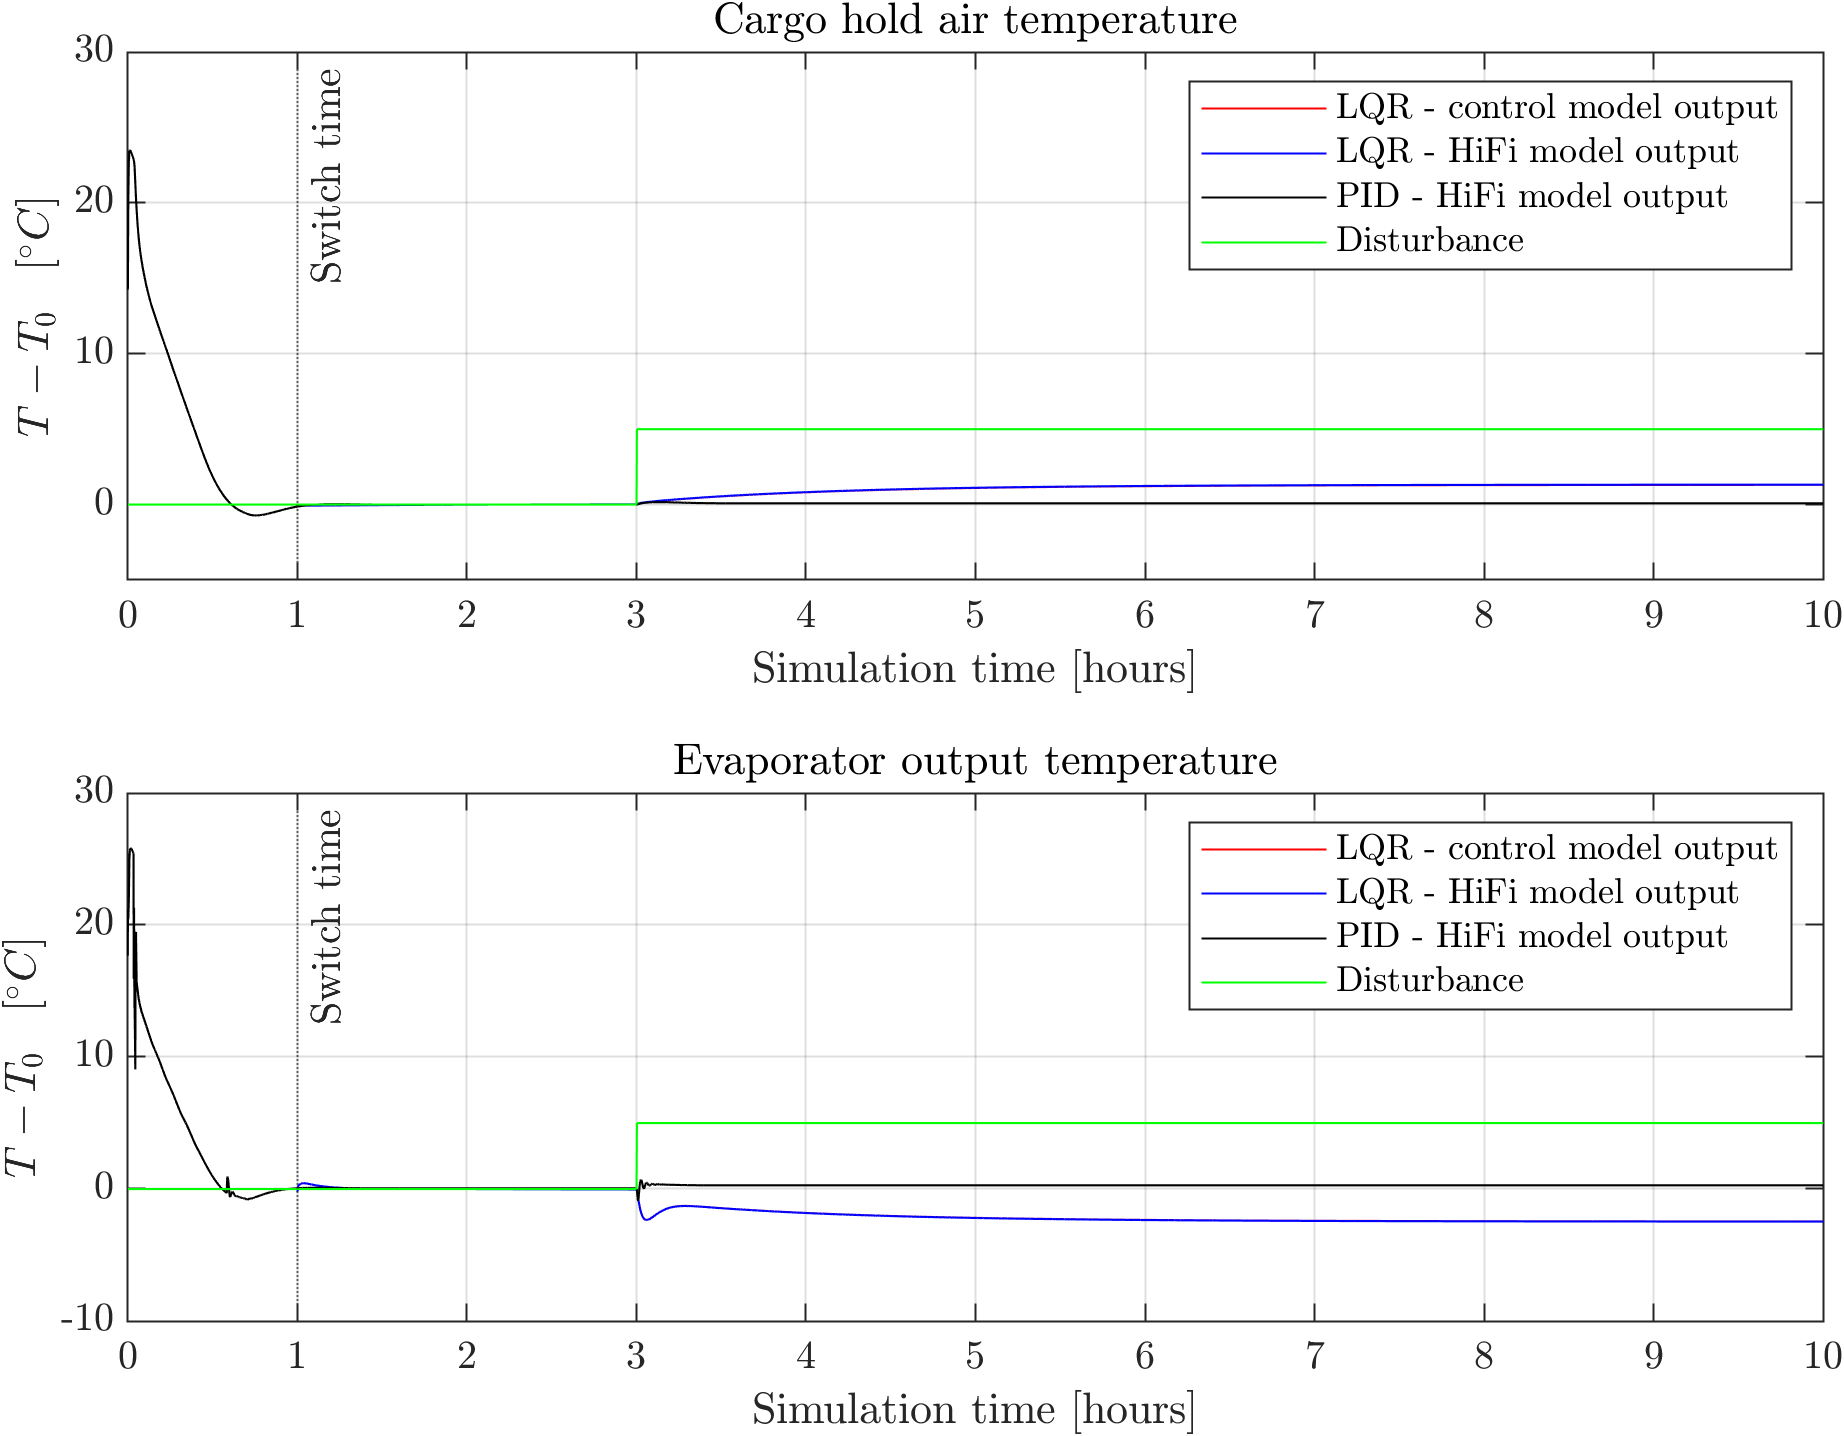
\includegraphics[width=0.8\textwidth]{Graphics/fig_LQRvsKresten_stepDist.png}
	\caption{Top: Cargo hold air temperature. $T_0$ = -4.25$^{\circ}$C. Bottom: Evaporator vapor refridgerant temperature. $T_0$ = -5.55$^{\circ}$C}
	\label{fig:LQR_wellTuned_5stepDist}
\end{figure}

\cref{fig:LQR_wellTuned_5stepDist_zoom} shows a zoomed in version of \cref{fig:LQR_wellTuned_5stepDist}, where the steady state error of the two outputs is seen.\\

\begin{figure}[H]
	\centering
	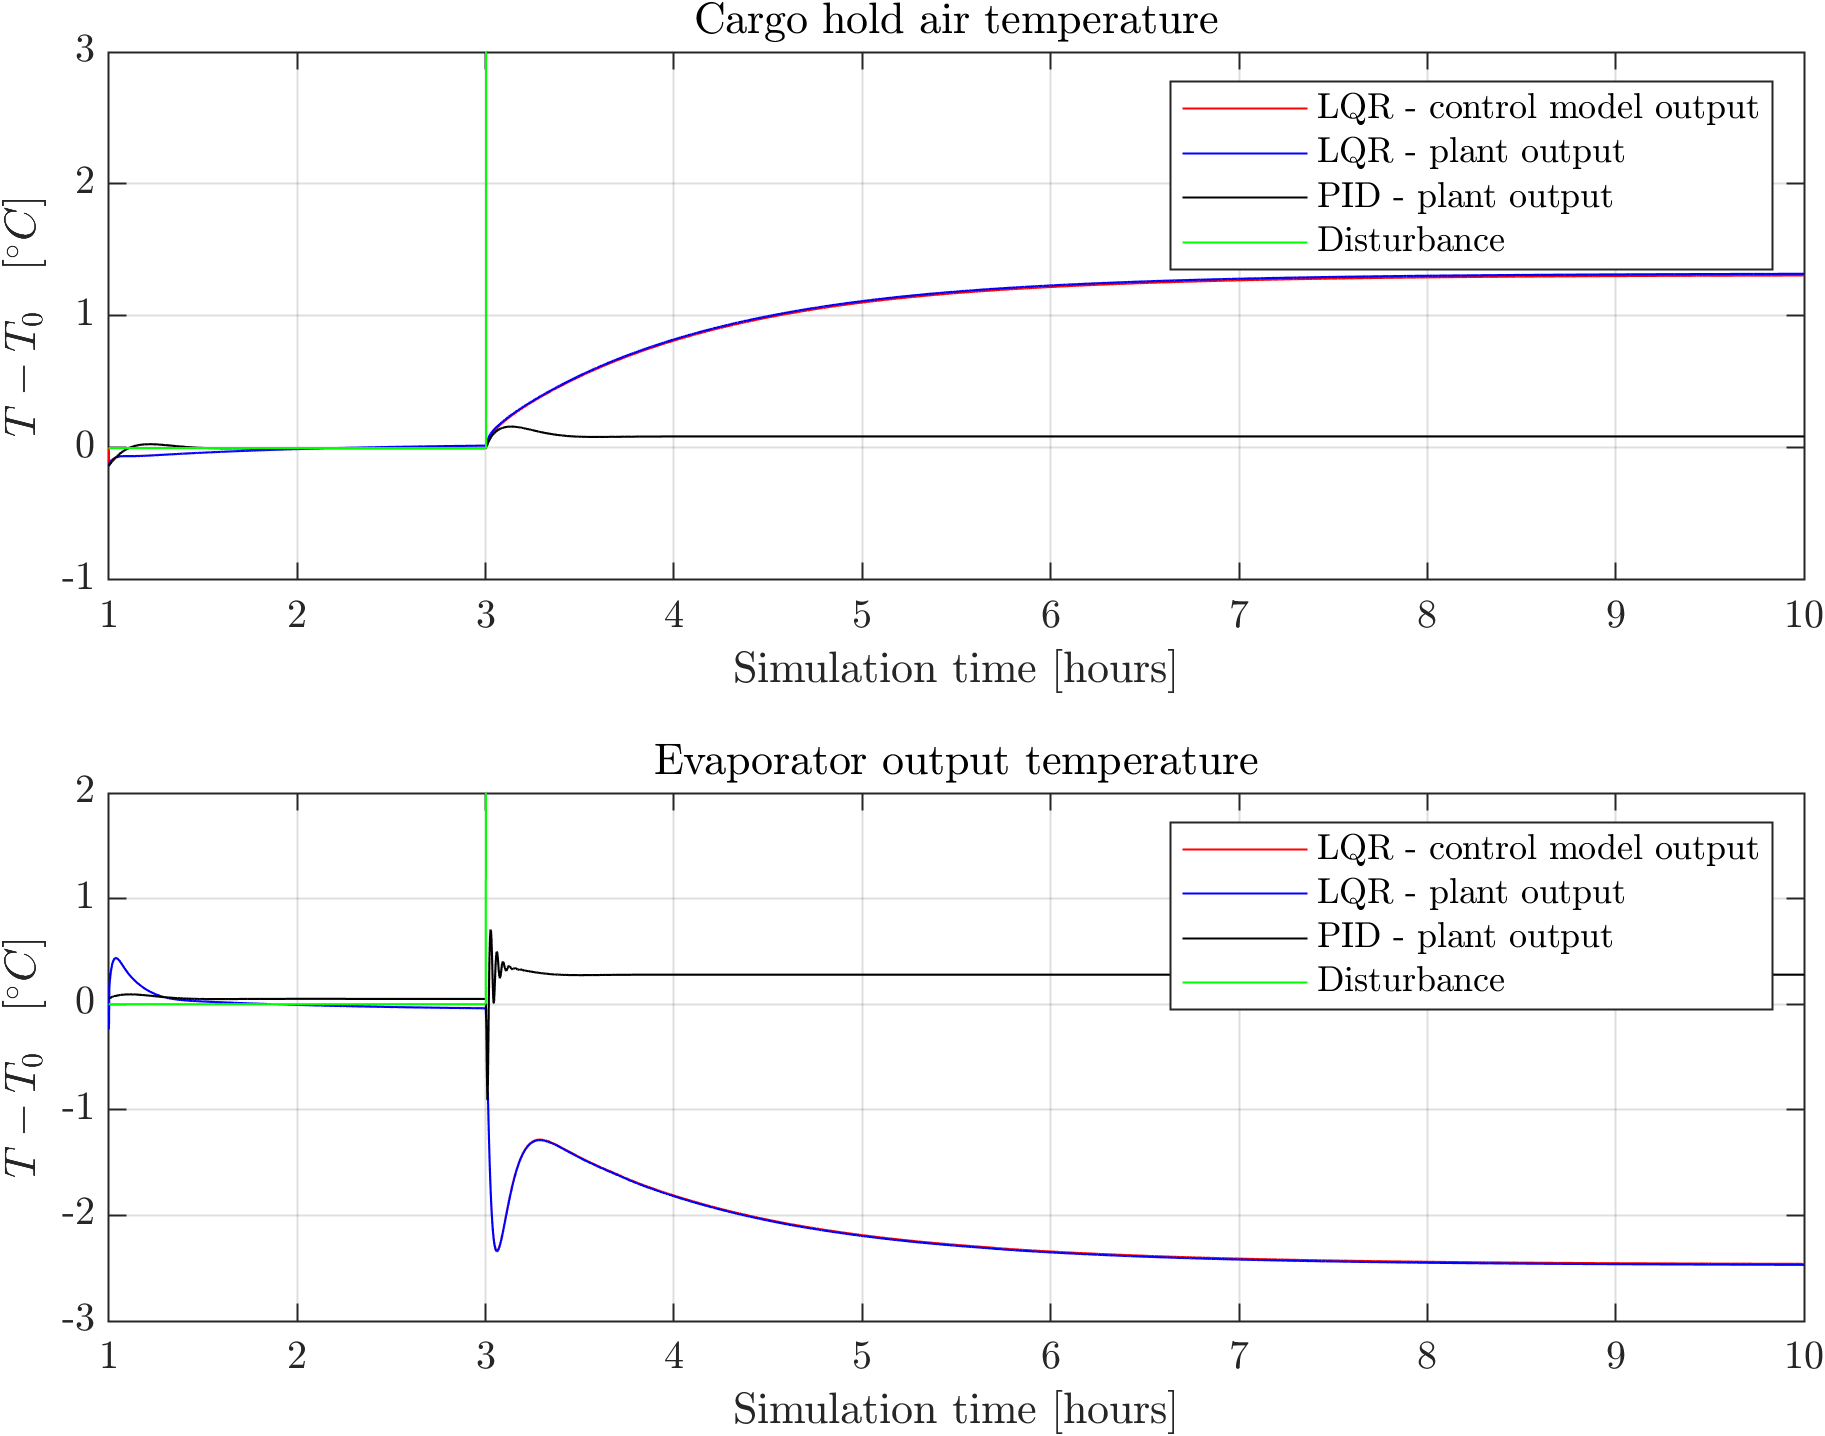
\includegraphics[width=0.8\textwidth]{Graphics/fig_LQRvsKresten_stepDist_zoom.png}
	\caption{Top: Cargo hold air temperature. $T_0$ = -4.25$^{\circ}$C. Bottom: Evaporator vapor refrigerant temperature. $T_0$ = -5.55$^{\circ}$C}
	\label{fig:LQR_wellTuned_5stepDist_zoom}
\end{figure}

It is seen that air temperature converges to 1.25$^{\circ}$C above the operating point, which means $T_{air} = -3^{\circ}C$. The superheat drops to 2.4$^{\circ}$C below the operating point, which means there is 3.6$^{\circ}$C superheat.\\

The increase in air temperature is large enough to be considered a problem for transportation of temperature critical goods, which is of course the intended purpose of the reefer trailer. The cause is likely, as was the case for the sine disturbance, that the controller is unable to change the compressor speed. The compressor speed is critical for increasing the refrigerant flow through the cycle, and is thus highly correlated with the cooling capacity of the system. \\

The drop in superheat is not as critical a problem as the air temperature. Ideally the controller would be able to keep it at the operating point, and in that context it is not desirable behavior. Technically, a drop in superheat increases the evaporation efficiency, and as long as there is a positive superheat no liquid will flow into the compressor. In summary, while the drop in superheat might increase efficiency without damaging the compressor, it would be a far more appealing if the controller was able to maintain the superheat at a fixed value.

The control inputs during this test is seen in \cref{fig:inputs_stepDist}.

\begin{figure}[H]
	\centering
	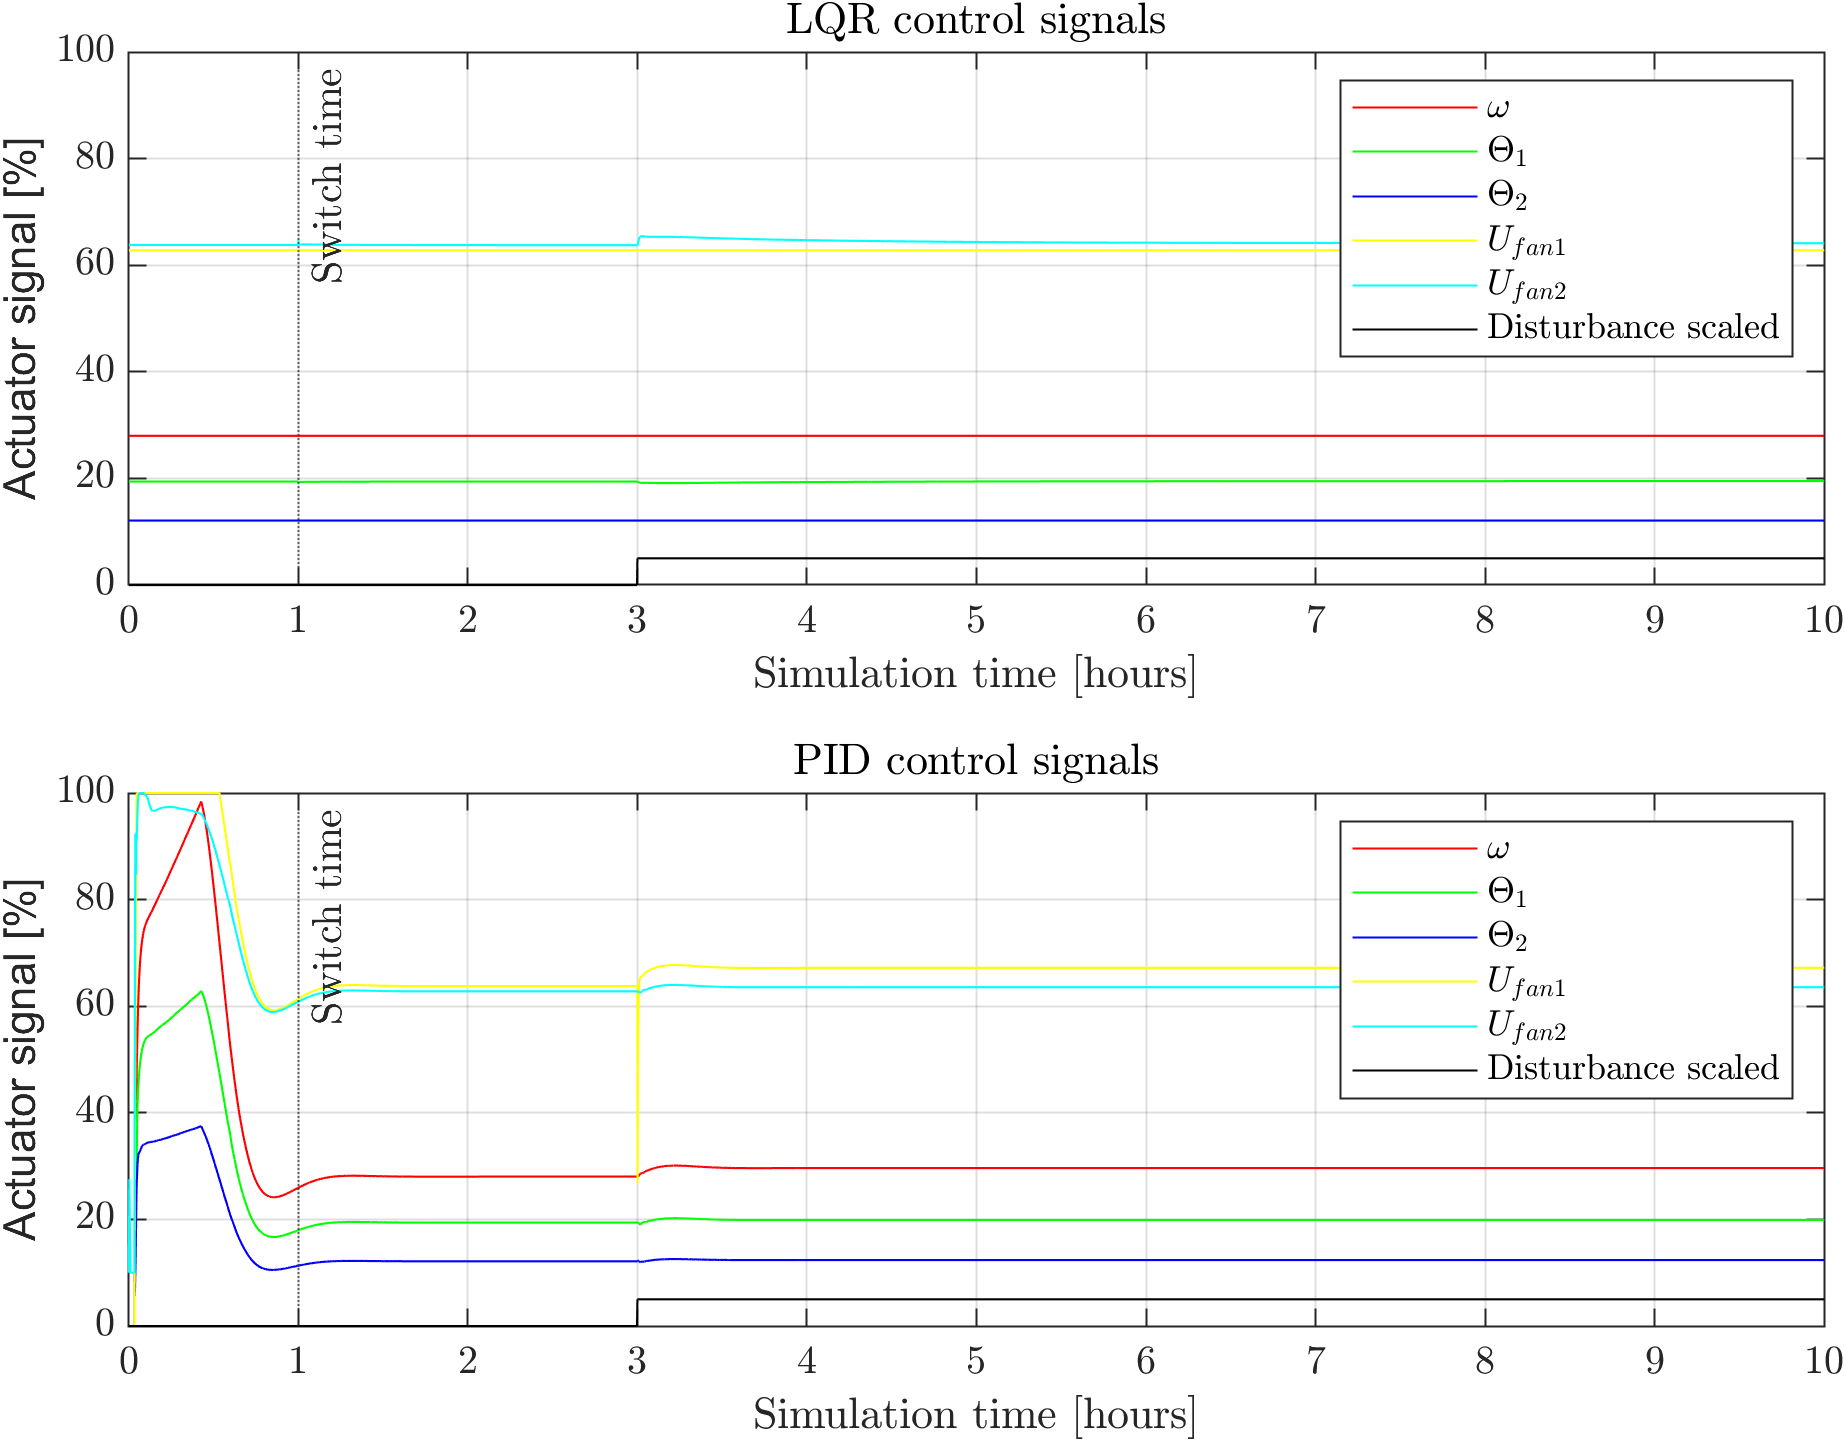
\includegraphics[width=0.8\textwidth]{Graphics/fig_inputs_stepDist.png}
	\caption{text}
	\label{fig:inputs_stepDist}
\end{figure}

\begin{figure}[H]
	\centering
	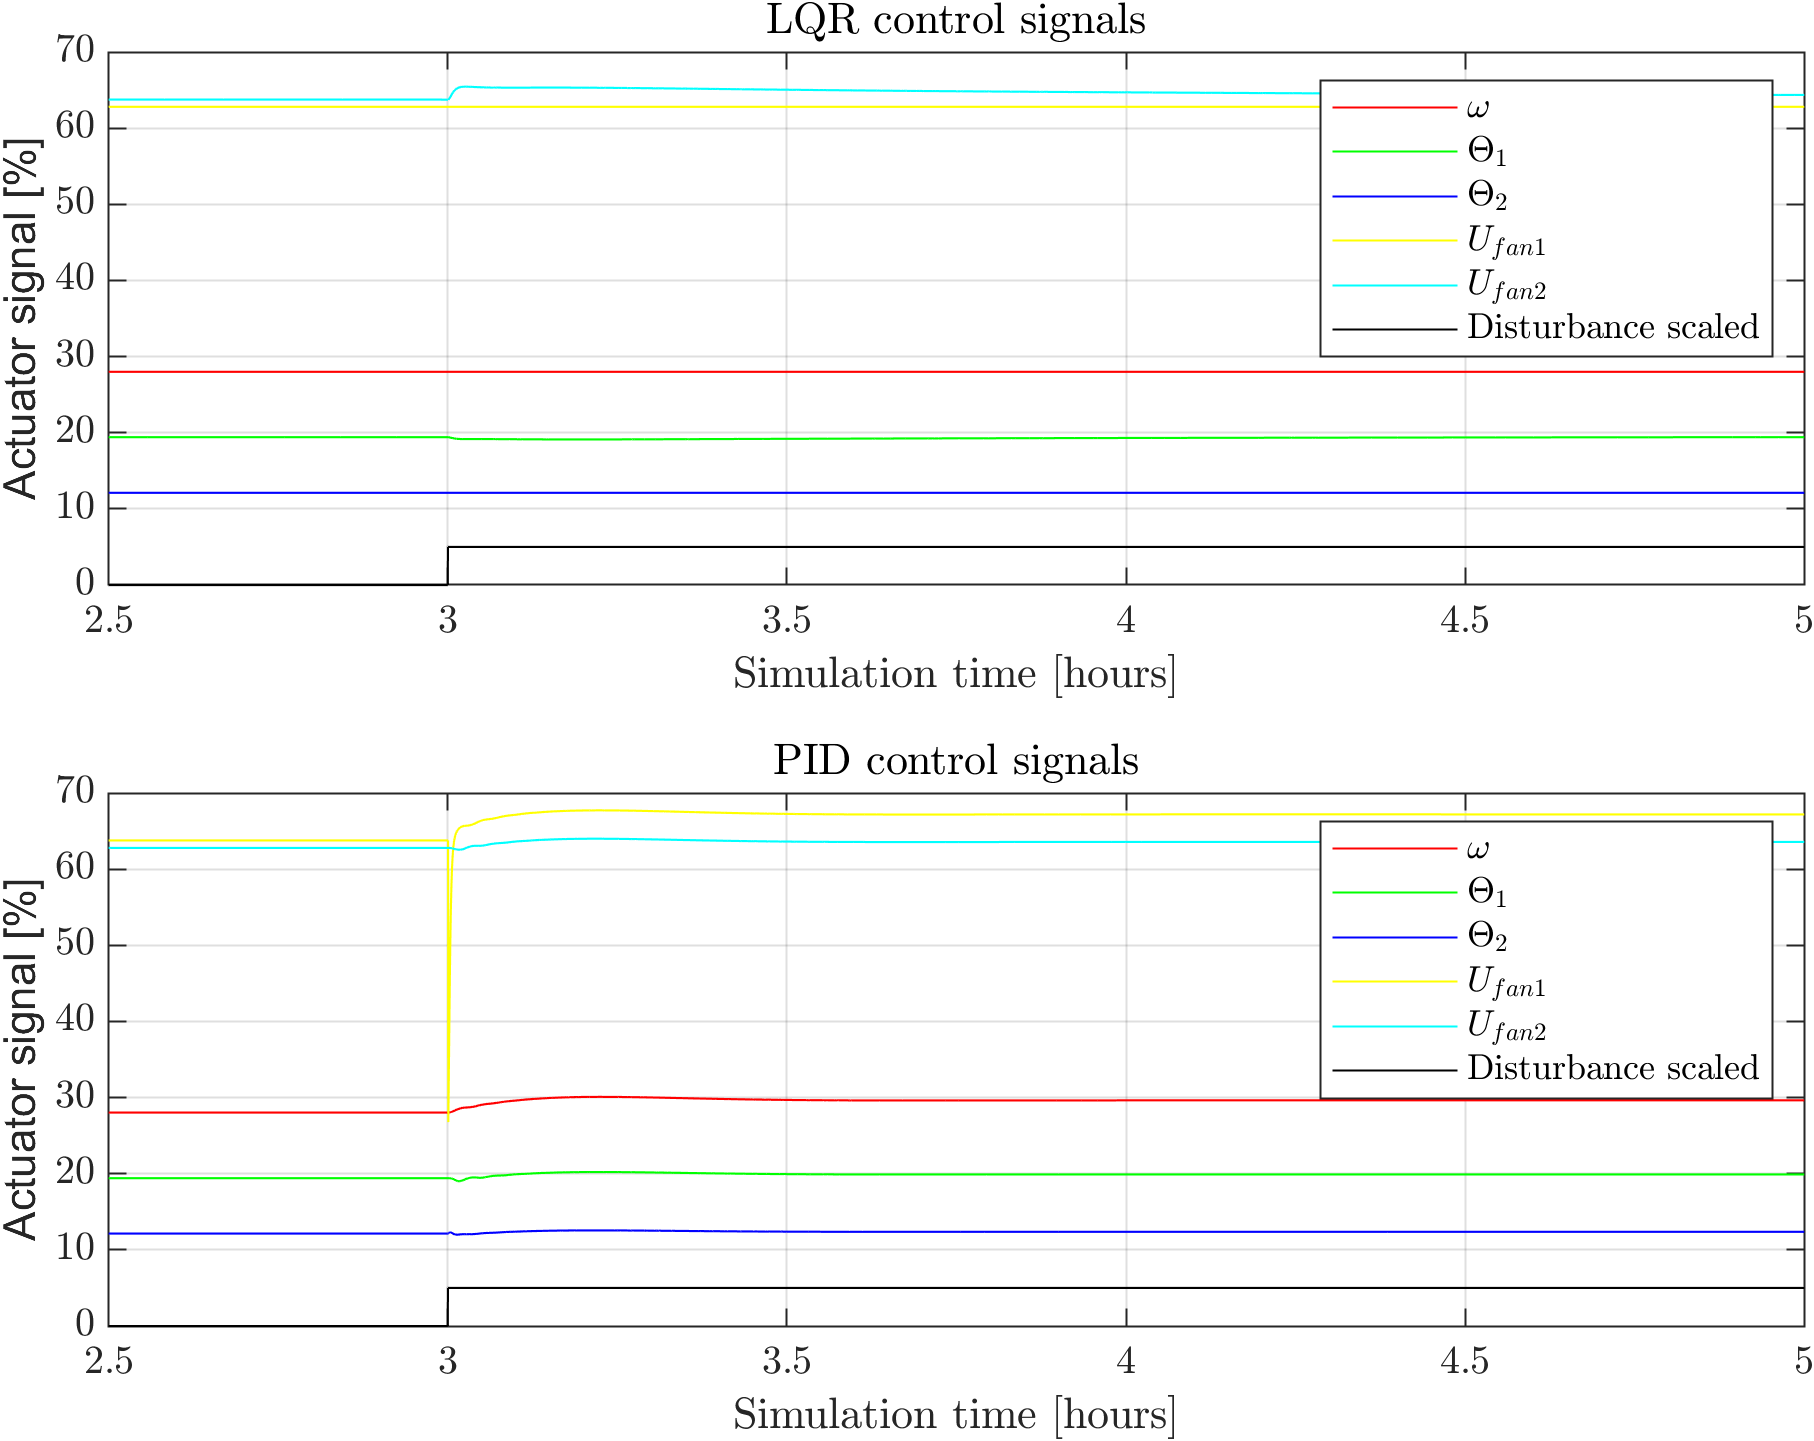
\includegraphics[width=0.8\textwidth]{Graphics/fig_inputs_stepDist_zoom.png}
	\caption{text}
	\label{fig:inputs_stepDist_zoom}
\end{figure}

\newpage
\subsubsection{Discussion}